\documentclass[10pt,letterpaper]{article}

\usepackage{cogsci}

\cogscifinalcopy % Uncomment this line for the final submission 


% \usepackage{pslatex}
% \usepackage{apacite}
\usepackage{float} % Roger Levy added this and changed figure/table
                   % placement to  for conformity to Word template,
                   % though floating tables and figures to top is
                   % still generally recommended!
% \documentclass[11pt,letterpaper]{article}
% \documentclass[11pt]{report}
% \documentclass{report}
% \documentclass{book}
\usepackage[hyperindex,bookmarks]{hyperref}
\hypersetup{
  colorlinks=true,
  allcolors=black
}
\usepackage{amssymb,amsmath}
% \usepackage{fullpage}
\usepackage{tabulary}
\usepackage{tabularx}

% \usepackage[margin=1.00in]{geometry}
% \usepackage[margin=0.90in]{geometry}

\usepackage{caption}
\usepackage{booktabs}
\usepackage{pslatex}
\usepackage{apacite}
\usepackage{subcaption}
\usepackage{pgfplots}
\usepackage{wrapfig}
\usepackage[english]{babel}
\usepackage{lmodern}
% \usepackage{setspace}
% \doublespace
% \usepackage{url}
\usepackage{bigfoot}
\usepackage[export]{adjustbox}
% \setlength\intextsep{0pt}
\setlength{\parskip}{0pt}

\usepackage{graphicx}

\title{Some forms of risk, cost, and uncertainty suppress social learning evolution}

\author{Team UncMod}

\begin{document}
\maketitle
\today


\begin{abstract}
  Social learning is essential to human and other species' survival. Given numerous
  existential threats facing humans, it is important to understand when social learning
  is beneficial---and when it is not. Current theory identifies risk and uncertainty
  as major factors that drive individuals to learn from others. However, in this paper, 
  we use agent-based modeling to demonstrate a surprising result: 
  sometimes risk and uncertainty leads to less frequent reliance on others,
  apparently because agents all have equally poor information, 
  apparently because others' 
  information is no better than our own.  Our analysis uses evolution to calculate
  optimal social learning frequency given a time-varying model environment with possibly
  dozens of behaviors performed by agents with varying life spans. 
  This work primarily builds on cultural evolution studies of social learning, 
  but it is highly relevant
  for cognitive science broadly to understand social cognition both (1)
  to understand why people behave the way they do---sociality is important for
  that; and (2) for the practical aim of designing autonomous 
  intelligent agents that learn from one another.

\textbf{Keywords:} social learning, evolution, culture, computation, optimization

\end{abstract}


\section{Introduction}


  \begin{itemize}
    \item 
      Social learning strategies specify \emph{when} , \emph{what}, and 
      \emph{from whom} one should learn~\cite{Laland2004,Kendal2018}.
    \item
      Many theories of social learning have demonstrated that social learning
      strategies, frequently specified \emph{a priori} by scientists or 
      others, can be adaptive under the right circumstances.
    \item
      In this paper we focus on understanding the \emph{when} of social learning, 
      specifically to understand which specific ecological conditions lead to greater or
      lesser social learning.
    \item
      Risk and uncertainty have been shown empirically to increase reliance on 
      socially-transmitted information, both in humans~\cite{Morgan2012,Mesoudi2014,Morgan2015}
      and non-humans~\cite{Carlier1997,Haun2012,Aplin2013,Aplin2015,Farine2015,Jones2015,Leris2016}
    \item
      Our work complements existing models and theories of social learning by 
      making payoff structures, life cycles, and environmental uncertainty 
      explicit, including the separation of vertical and horizontal social transmission.
    \item
      Furthermore, we are able to identify \emph{optimal} social learning strategies
      by allowing the frequency of horizontal social learning and the magnitdue
      of vertical social learning to evolve over a continuous range of values.
    \item
      This work strengthens our understanding of the cognitive and cultural factors
      that underlie social learning, and possibly provides practical solutions
      for engineering online collective, adaptive intelligent systems.
    \item
      This understanding in turn can be used to improve human outcomes by 
      identifying when social learning is objectively beneficial or not, independent
      of the various cognitive biases that sometimes lead us to follow others when 
      the information provided by others may be misleading, or vice versa.
    \item
      Understanding how people behave in different risk and uncertainty
      scenarios can help us in designing interventions for countering
      existential threats such as pandemics and climate change~\cite{Jones2021}.
  \end{itemize}

\subsection{Cultural evolution of social learing}
    \begin{itemize}
      \item 
        Social learning is an adaptive strategy for identifying beneficial behaviors.
      \item
        Consensus in cultural evolutionary theory of social learning focuses on
        identifying various strategic modules that may act independently or
        in concert~\cite[see Figure 1]{Kendal2018}.
      \item
        Cultural evolutionary theories of social learning are based on human
        and non-human empirical studies.
      \item
        These theories and their empriical support are reviewed below.
    \end{itemize}

    \subsubsection{Cultural evolutionary social learning theories}
    \begin{itemize}
      \item
        What is cultural evolution and why is it valuable for studying social
        learning?
      \item 
        \citeA{Rogers1988} consolidated existing theory and showed how 
          \begin{enumerate}
            \item 
              Environmental uncertainty
            \item
              ``Costly'' individual learning 
          \end{enumerate}
        contribute to social learning, but found that genetic evolution led to
        the situation where social learning did not enhance fitness, i.e.,
        that culture is nonadaptive~\cite{Enquist2007}.

      \item
        \citeA{Feldman1996} \citeA{Boyd1988}
        
      \item
        \citeA{Enquist2007} show that social learning may be adaptive if
        individuals adopt \emph{conditional} social
        learning. The condition used by individuals is specified by the
        authors: their model assumes individuals may first try social learing,
        but then use individual learning if social learning fails, which could
        be called \emph{critical social learning}. 
      \item
        \citeA{Rendell2009} expand the possible social learning strategies to
        consider four total: pure social learning, pure individual/asocial
        learning, critical social learning \cite{Enquist2007}, and
        \emph{critical individual/asocial learning}. 
      \item
        \citeA{Perreault2012} provide the first approach to enable
        \emph{adaptive} heuristic strategies that specify \emph{when}, i.e.,
        \emph{how frequently} individuals use social learning to select their
        behavior.
      \item
        \citeA{Rendell2010} used crowdsourcing to identify optimal social
        learning frequencies. They also incorporated environmental uncertainty
        within a multiarmed bandit framework by allowing payoffs to change
        probabilistically within each round, which they note may be impossible to
        optimize analytically~\cite{Papadimitriou1999}.
    \end{itemize}

    \subsubsection{Empirical support for evolutionary social learning theories}
    \begin{itemize}
      \item 
        Human
        \begin{itemize}
          \item 
            \citeA{Morgan2012} operationalizes many (WHICH) of the conjectures 
            about the role of social learning in a series of behavioral 
            studies with different tasks (THAT REVEALED WHAT?)
          \item
            \citeA{Mesoudi2014} studied differences in social learning between
            Chinese and Westerners.
          \item
            \citeA{Morgan2015} and \citeA{Shneidman2016} studied social learning
            during human developmental periods.
        \end{itemize}
      \item
        Non-humans
        \begin{itemize}
          \item 
            \citeA{Carlier1997} found that ``ecological differences'' led to
            ``differences in social learning between adjacent, mixing populations
            of Zenaida doves. \citeA{Aplin2013,Aplin2015} found social learning is essential for
            wild birds to provide a consistent food supply for themselves, but
            more stress in early life leads to more social learning (among
            zebra finches, specifically)~\cite{Farine2015}.
          \item
            \citeA{Haun2012} chimps, orangutangs, human children
          \item
            \citeA{PatriciaJones2015} social learning in honeybees
          \item
            Guppies learn socially to different degrees depending on 
            ``age and early social environment'' \cite{Leris2016}
        \end{itemize}
    \end{itemize}

    \subsection{Agent-based modeling}

\subsection{Overview and plan}

In the next section we enumerate our agent-based model of behavior selection and
social learning evolution, including how we used our model to construct
computational experiments that induce changes in the evolution of social learning 
dependent on systematically varied risk, cost, and uncertainty variables.
Then in the Analysis section we show that, indeed, some forms of risk, cost, 
and uncertainty lead to lower levels of social learning. We also show that 
social learning increases when environmental uncertainty increases, so our model
agrees with existing theoretical predictions that tend to operationalize 
uncertainty that way. Finally, we explain how we have indeed provided important 
counterexamples to the rule that increased risk, cost, or uncertainty lead to
increased social learning; our counterexamples come in the form of testable
predictions that can be followed up by expanded models using our framework and
behavioral studies to see if human or other species' behavior matches or diverges
from these predictions.


\section{Model}

We developed an agent-based model of a society of $N$ who individually must decide
which of $B$ behaviors to perform at each time step. Each behavior is a ``bandit'',
a common model component to generically represent behaviors with probabilistic
payoffs~\cite{Rendell2010}. Bandits are like slot machines in a casino. Each
bandit/behavior $b$ yields a payoff of 1 with probability $\pi_b$, 
which is also the expected payoff of behavior $b$. Agents decide which behavior
to do at each time step based either on social information with probability $s$
or asocial information with probability $a = 1 - s$. We operationalized uncertainty
and risk in four different ways: (1) the probability the optimal behavior changes
from one generation to another, environmental uncertainty $u$; (2) the difference
between the optimal expected payoff behavior $\pi_{high}$ and the expected payoff
of the other behaviors, $\pi_{low}$; (3) the number of possible behaviors, $B$;
and (4) the life span, or time steps per generation, $M$. Over $R$
rounds/generations of $M$ time steps, agents die off and reproduce.
Those selected to reproduce pass on their social learning frequency $s$ with
mutation, so that selection operates to maximize payoffs by favoring higher payoff
individuals for reproduction. We developed a series of computational experiments
where we systematically vary the uncertainty and risk variables and observe the
social-asocial learning difference, our primary outcome measure, $s - a$. In this
section we explain each of these steps in detail so the reader understands how we
came to our conclusion that increased uncertainty and risk sometimes suppress social
learning.


\subsection{Agents}

In each simulation, $N$ agents---autonomous intelligent problem solvers---
select which behavior to perform based on either social or asocial
information (Figure~\ref{fig:behaviorSelection}). 
Whether asocial or social information is used, the agent tracks 
the mean payoff of each behavior $b$, denoted $\bar\pi_b$, and a \emph{count} 
of how many times it has performed each behavior, denoted $c_b$. Mean payoffs
are updated from $\bar\pi_b$ to $\bar\pi_b'$ using exponential weighted averaging, 
$\bar\pi_b' = \bar\pi_b + \frac{\mathrm{Bandit(0, 1)} - \bar\pi_b}{c_b'}$, where
$\mathrm{Bandit(0, 1)}$ is 0 or 1 depending on the result of the bandit draw.

Agents choose social information with probability $s$, which agents inherit from their
parents with mutation. Since agents can only choose social or asocial information in
our model, the probability of using asocial information for behavior selection is
$a = 1 - s$. If an agent selects uses social information for behavior selection
the agent first selects $N_T$ potential teachers at random from the other
$N-1$ agents in the population ($N_T = 3$ in the example on the bottom of 
Figure~\ref{fig:behaviorSelection}). The agent adopts one of the potential 
teachers' behaviors at random, weighted by each potential teacher's accumulated
payoffs in the round. 

If an agent uses asocial information the agent selects a
behavior at random, weighted by the
softmax function applied to that behavior's observed mean payoff relative to 
all mean payoffs: 
$\Pr(\text{do behavior }b) = 
  \frac{\exp(\bar\pi_b / \tau) }{ 
\sum_{b=1}^B \exp(\bar\pi_b / \tau)}$.
The softmax method is used because it enables agents to explore alternative
behaviors sometimes and exploit the best observed behavior other times.
Softmax may be a suitable,
biologically plausible model for the process by which humans identify structure in
problems such as these~\cite{Schulz2019,Gershman2019}. To mimic increased plasticity
and exploration in the developmental
period in humans we use simulated annealing to decrease $\tau$ over the course of a
model generation (REF GOPNIK?).

\begin{figure}
  \centering
  \caption{\textbf{Behavior selection.} 
    Agents select a behavior to do at each timestep either using asocial 
  information (top row) with probability $a$ or social information with
probability $s = 1 - a$ (bottom row). (WILL EDIT TO MAKE TEXT LARGER/MORE
READABLE)}
  \label{fig:behaviorSelection}
    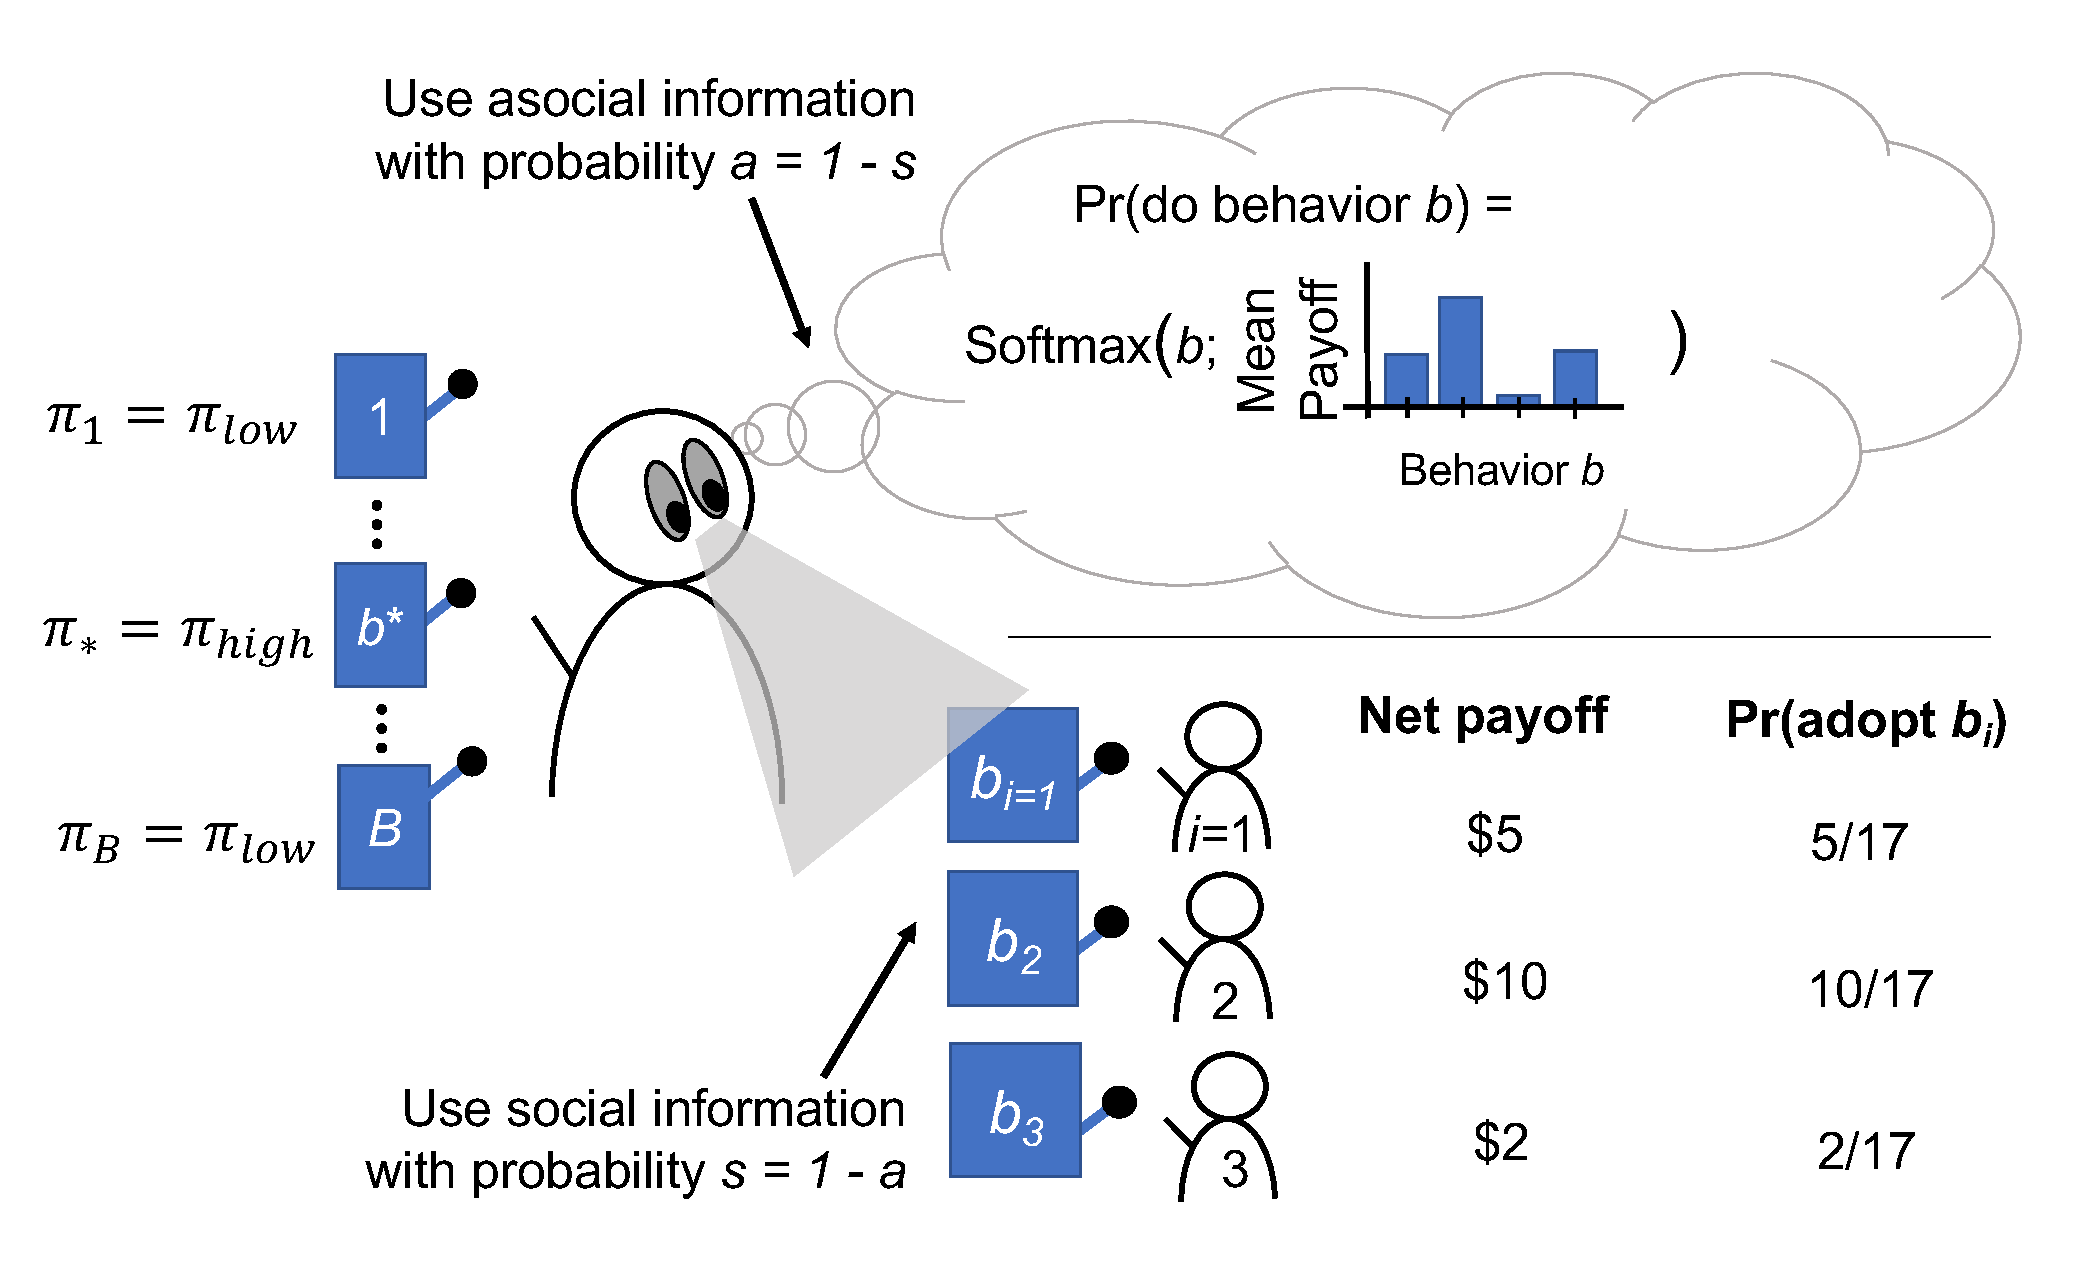
\includegraphics[width=0.515\textwidth]{Figures/BehaviorSelection.pdf}
\end{figure}




\subsection{Uncertainty and risk parameters: payoff structure and variation, behavioral affordances, and life expectancy}

In our model, uncertainty, risk, and cost are not assumed or imposed in our model, 
but instead are a consequence of model parameters that structure the behaviors
agents can do: (1) the expected payoffs the agents receive, 
(2) how frequently the optimal behavior changes, i.e., the \emph{environmental
uncertainty}; (3) the number of behaviors 
afforded by the environment; and (4) how many time steps 
agents exist before they possibly reproduce and definitely die off.

Payoffs are structured as follows: 
one of the $B$ behaviors yields payoff $\pi_{high}$; the rest yield expected payoffs
$\pi_{low}$. Recall that each behavior yields a payoff of 1 with probability
$\pi_{high/low}$, and 0 otherwise. 
$B$ itself is once source of uncertainty or cost since it would
take an agent longer on their own to determine which behavior is optimal. 
We further define the following measure of uncertainty or difficulty introduced when
low and high payoffs are more similar, making it more difficult to discern which
behavior is the optimal one. We define \emph{payoff ambiguity} as
\begin{equation}
\Delta \pi = \frac{1}{\pi_{high} - \pi_{low}} - 1,
\end{equation}
which is 0 when $\pi_{high} = 1$
and $\pi_{low} = 0$, and goes to $\infty$ as $\pi_{low} \to \pi_{high}$.

To model \emph{environmental uncertainty}, we switch which behavior is optimal
to another randomly-selected behavior with probability $u$ after every generation.

Finally, the number of steps per generation/round, $M$, effectively increases the
importance of each time step for acquiring payoffs. $M$ can be thought of as a
lifespan since agents are subject to selective reproduction and die off after 
$M$ time steps. In that case, smaller values of $M$ would represent greater risk,
such as predation risk. In terms of uncertainty, 
at the end of the generation agents are less certain about which behavior is best
when $M$ is smaller than when it is larger.


\subsection{Dynamics and evolution}

Model dynamics occur on two timescales. The smaller time scale is the time step.
There are $M$ time steps per generation/round, analogous to a biological generation, 
after which the agents reproduce with probability proportional to their 
accumulated payoffs in the round relative to the others, 
followed by whole-population die-off. 

Children inherit their parent's social learning frequency $s$ and vertical
transmission magnitude, $v$, defined now. Our model includes vertical information
transmission from parent to children agents in the form of 
the parent's record of mean behavior payoffs $\bar\pi_b$ and number of observations
of each behavior by the parent, $c_b$. 
The vertical transmission magnitude mediates the information content in
vertical transmissions, which is also allowed to evolve to 
optimize vertical transmission along with social learning frequency. Children learn
their parent's observed mean payoff histograms according to this rule: 
$\bar\pi_b' = \bar\pi + v(\bar\pi_b - \bar\pi)$, 
where $\bar\pi_b'$ is the mean payoff transmitted to the child, 
$\bar\pi_b$ is the mean payoff in the parent's memory, and $\bar \pi$ is the 
mean payoff across all behaviors observed by the parent.

Agent traits $s$ and $v$ are passed from parents to children with a mutation drawn
from a normal distribution with mean, $\mu = 0.1$ for this paper's analysis.
If this causes either trait to become less than 0 the trait value is remapped to
0; if the value is greater than 1 it is remapped to 1. Agents are selected
with replacement, with probability proportion to their net payoffs, to generate
$N$ child agents to replace the existing agents, all $N$ of whom die off 
(Figure~\ref{fig:evolution}).

\begin{figure}
  \caption{\textbf{Evolution.} Selection occurs every $M$ time steps.
  Example population with $N=5$ agents shown. All agents die off at the end of
their generation, marked with a cross. Reproducing agents, marked with a circle, 
are sampled with replacement with probability of selection proportional to their 
accumulated payoffs. Child agents inherit their parent's social learning
frequency with mutations.}
  \label{fig:evolution}
  \centering
    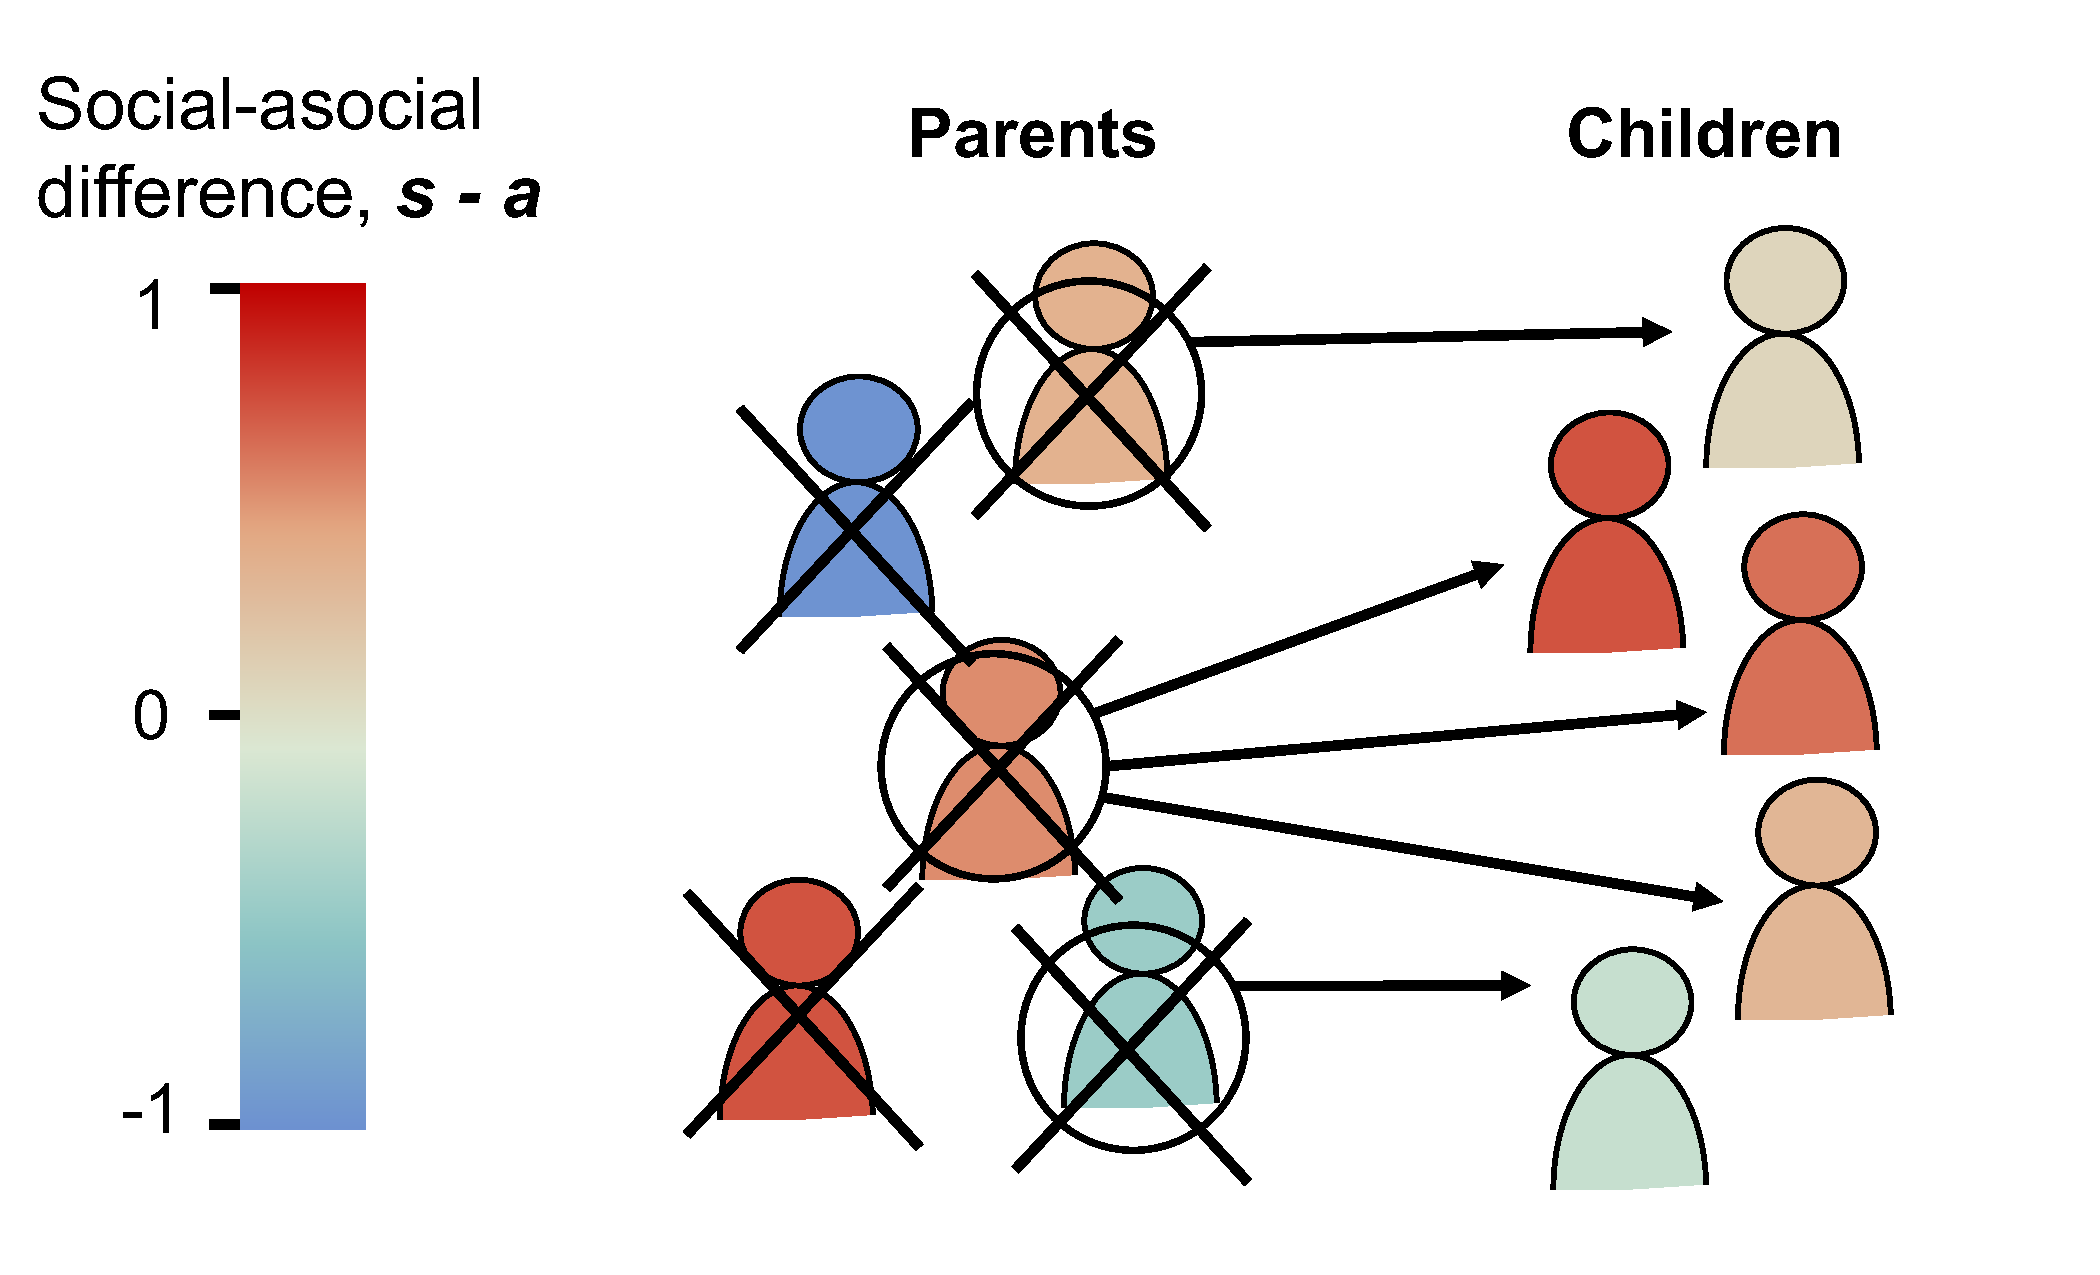
\includegraphics[width=0.45\textwidth]{Figures/Evolution.pdf}
\end{figure}


\subsection{Computational experiments}

We combine the elements above to create computational experiments that observe
changes in our main outcome variable, social-asocial learning difference $s - a$
as we systematically vary the independent 
uncertainty/risk/cost variables $B$, $\Delta \pi$,
$M$, and $u$. The goal of these experiments is to test whether social learning
increases, decreases, or changes non-monotonically as we vary the 
independent variables.

For each parameter setting in our analysis we caluculated the average value of
$s-a$ across 100 trial runs, across all agents in the simulation, 
over the last 20,000 of $T = 100,000$ simulation time steps.

We analyze our experiments in two Analysis sections below, using results from
three computational experiments. In the first experiment we systematically co-varied
the base payoff $\pi_{low} \in \{0.1, 0.2, \ldots, 0.8\}$, the optimal payoff 
$\pi_{high} \in \{0.2, 0.3, \ldots, 0.9\}$;
in the Analysis below we also use data from this experiment to analyze 
the effect of environmental uncertainty, which was varied over the values 
$u \in \{0.0, 0.1, 0.25, 0.5, 0.75, 0.9\}$. In the second experiment, we 
co-varied the number of possible behaviors, $B \in \{10, 20, \ldots, 100\}$, 
along with uncertainty $u \in \{0.1, 0.9\}$. In the final experiment, we 
co-varied the lifespan of agents, the number of steps per generation, 
$M \in \{5, 10, 20, 50, 100\}$ and the environmental uncertainty $u \in \{0.1,
0.9\}$.


\subsection{Implementation}

The model was implemented in Julia using the Agents.jl package for model development
and the Gadfly package for figures. Simulations were run on the Sherlock supercomputing
cluster at Stanford University. Model and analysis code, and links to output 
datasets used for this paper's figures, can be found 
at \url{https://github.com/mt-digital/UncMod}.


\section{Analysis}


We now analyze the results of our computational experiments that show certain forms
of uncertainty lead to less frequent social learning, which had not previously been
predicted by current theory. We also show that increased environmental
uncertainty between generations leads to more more frequent social learning,
which is consistent existing theories. We show that differences in behavioral payoffs
are the most significant independent variable we tested. We also tested the effect
of two other independent variables found to have less significant effects on
social learning frequency: (1) the number of time steps per generation, analogous i
to lifespan; and (2) the number of behaviors allowed by the environment. 
We will measure the frequency of social learning by the differential between
social learning frequency and asocial earning frequency, denoted $s - a$ where
$s$ is the average social learning frequency at equilibrium and $a$ is the 
asocial learning frequency at equilibrium. We first show that $s-a$ actually
increases as payoff ambiguity ($\pi_{high} - \pi_{low}$), a form of ``uncertainty'',
decreases, contrary to current expectations. In other contexts, however, 
payoff ambiguity and $s-a$ are positively correlated as existing theory would
suggest. We then perform a sensitivity analysis over the two other independent
variables tested, the number of time steps per generation, $M$, and the number
of behaviors the environment affords, $B$.
 
\subsection{Social learning frequency variation over payoff 
  ambiguities and environmental uncertantites}
  \vspace{0.5em}

In this section we show results from our primary computational experiment that
shows social learning frequency is not always positively correlated with 
all forms of uncertainty. However, we also use this experiment's output data
to show that our model predictions agree
with existing theoretical predictions, in that intergenerational uncertainty 
tends to increase dependence on social learning.


\subsubsection{Social learning and payoff ambiguities}

Across low (Figure~\ref{fig:expectedPayoffHeatmaps_low}) , moderate
(Figure~\ref{fig:expectedPayoffHeatmaps_med}), and high
(Figure~\ref{fig:expectedPayoffHeatmaps_high}) levels of environmental
uncertainty we see counterexamples to the general rule that ``uncertainty''
generally leads to greater reliance on social learning when uncertainty is
operationalized as payoff ambiguity we define as 
$\Delta \pi = \frac{1}{\pi_{high} - \pi_{low}}
- 1$. This measure is useful because it is 0 when payoffs are maximally 
different, $\pi_{high} = 1$ and $\pi_{low} = 0$, and goes to $\infty$ when
$\pi_{high} = \pi_{low}$. If $\Delta \pi$ represents uncertainty, then as 
ambiguity $\Delta \pi$ decreases, social learning frequency should also decrease 
compared to contexts with greater ambiguity. However we found several counterexamples
where social learning was more favored when ambiguity was lower.
One example where social learning frequency incerases when ambiguity decreases
is with low environmental uncertainty and $\pi_{high} = 0.9$,
social learning frequency decreases while $\pi_{low}$ and $\Delta \pi$ 
increase (Figure~\ref{fig:expectedPayoffHeatmaps_low}).
With moderate and high environmental uncertainty, and with $\pi_{low} = 0.1$
for example, social learning frequency also increases as $\pi_{high}$ increases
and ambiguity $\Delta \pi$ decreases (Figures~\ref{fig:expectedPayoffHeatmaps_med}
and~\ref{fig:expectedPayoffHeatmaps_high}). 

\begin{figure}

  % \centering
  \caption{Average difference in social and asocial learning frequencies, $s - a$, over
  different payoff structures defined by bandit payoffs $\pi_{high}$ and $\pi_{low}$
for three levels of environmental uncertainty. $B = 50$, $M = 20$.}
  \label{fig:expectedPayoffHeatmaps}

  \begin{subfigure}[b]{0.5\textwidth}
    % \centering
    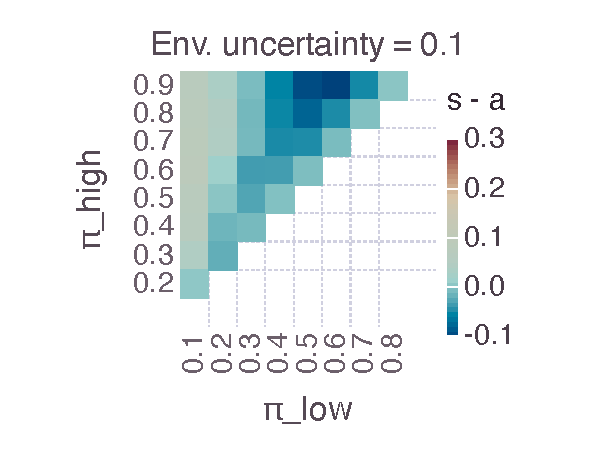
\includegraphics[width=0.7\textwidth]{Figures/expected-payoff-heatmap_envUnc0p1.pdf}
  \caption{Low environmental uncertainty}
  \label{fig:expectedPayoffHeatmaps_low}
  \end{subfigure}
  \begin{subfigure}[b]{0.5\textwidth}
    % \centering
    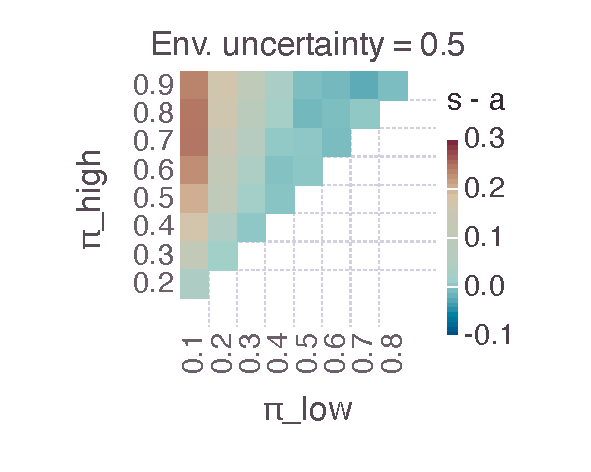
\includegraphics[width=0.7\textwidth]{Figures/expected-payoff-heatmap_envUnc0p5.pdf}
  \caption{Moderate environmental uncertainty}
  \label{fig:expectedPayoffHeatmaps_med}
  \end{subfigure}
  \begin{subfigure}[b]{0.5\textwidth}
    % \centering
    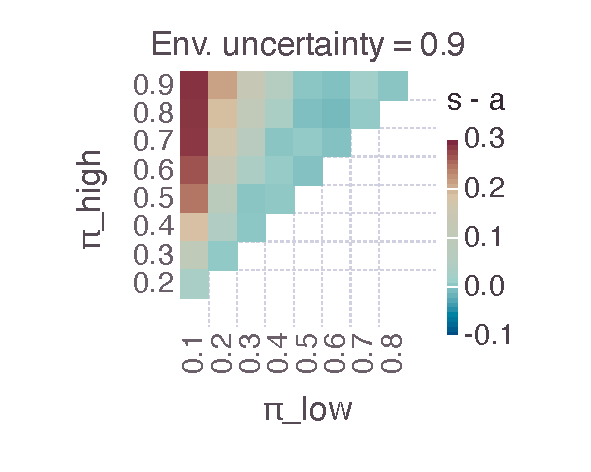
\includegraphics[width=0.7\textwidth]{Figures/expected-payoff-heatmap_envUnc0p9.pdf}
  \caption{High environmental uncertainty}
  \label{fig:expectedPayoffHeatmaps_high}
  \end{subfigure}
  
\end{figure}


\subsubsection{Environmental uncertainty increases social learning frequency}

We now examine changes in social learning frequency as a function of environmental
uncertainty to demonstrate our model is consistent with existing theory that
predicts social learning frequency should increase with environmental 
uncertainty, since horizontally transmitted information is more frequently
made obsolete when environmental uncertainty is greater. Indeed our model predeicts
that social learning frequency increases with environmental uncertainty
(Figure~\ref{fig:environmentalUncertainty})
for two of the most sensitive payoff structures identified in the previous
analysis.

\begin{figure}
  \centering
  \caption{Our model predicts social learning frequency increases with environmental
  uncertainty for two of the most environmental uncertainty-sensitive payoff
  structures revealed by the above analysis. $B = 50$, $M = 20$.}
  \label{fig:environmentalUncertainty}
    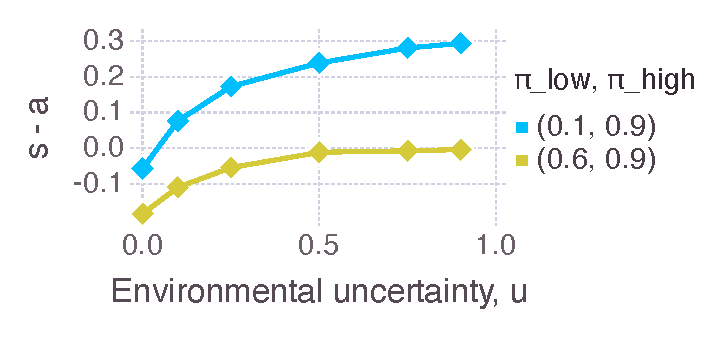
\includegraphics[width=0.4\textwidth]{Figures/s-a_overEnvUnc.pdf}
\end{figure}

\subsection{Behavioral affordances, decreased life span suppress social learning}
We can operationalize two other model factors so far set constant 
that could be interpreted as uncertainty: (1) the number of behavioral affordances
provided by the environment in the form of the number of ``bandits'' in the model;
and (2) the ``life span'' of agents, i.e.\ the time of existence of each generation, 
represented by the number of time steps per round. In this section of our analysis
we first systematically varied the number of possible behaviors $B$, then 
systematically varied the life span $M$, and again observed the resulting 
difference between social and asocial learning frequencies $s - a$. In the case
of low environmental uncertainty $B$ has no effect on
(Figure~\ref{fig:nbehaviors0p1}); however, with high environmental uncertainty
we observe another counterexample to the maxim ``copy when uncertain'' since
as $B$ increases, social learning frequency decreases
(Figure~\ref{fig:nbehaviors0p9}). The life span, represented by $M$, had a weak,
non-monotonic effect on $s-a$---an insignificant effect, though, 
compared to environmental uncertainty and payoff structure
(Figure~\ref{fig:steps_per_round}).

% $s-a$ on $B$ and $M$ are less significant than payoff ambiguity
% $\Delta \pi$. 

\begin{figure}

  \centering
  \caption{Social-asocial learning difference $s-a$ over number of possible behaviors,
  $B$, and environmental uncertainty, $u$. $s-a$ depends on $B$ under high
  environmental uncertainty, but environmental uncertainty and payoff structure 
  are more significant factors than $B$. $M = 50$.}

  \label{fig:nbehaviors}

  \begin{subfigure}[b]{0.35\textwidth}
    \centering
    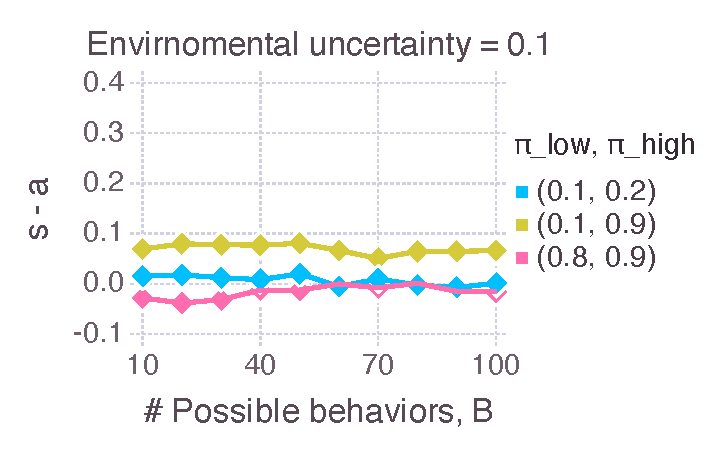
\includegraphics[width=\textwidth]{Figures/nbehaviors0p1.pdf}
  \caption{Low environmental uncertainty}
  \label{fig:nbehaviors0p1}
  \end{subfigure}
  \begin{subfigure}[b]{0.35\textwidth}
    \centering
    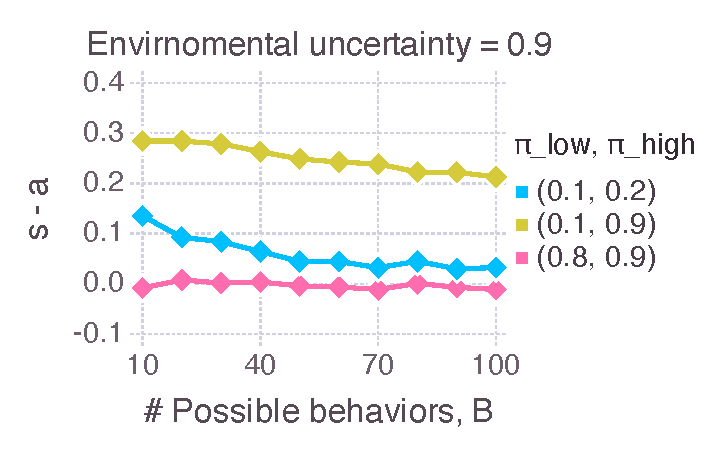
\includegraphics[width=\textwidth]{Figures/nbehaviors0p9.pdf}
  \caption{High environmental uncertainty}
  \label{fig:nbehaviors0p9}
  \end{subfigure}
  
  
\end{figure}



\section{Discussion}
 
In this paper we set out to demonstrate that certain operationalizations of
uncertainty result in counterexamples to the observed rule that social learning
should be favored when uncertainty increases. Indeed we showed that 
uncertainty in the forms of increased payoff ambiguity, increased number 
of possible behaviors, and increased lifespan (decreased ``risk'' of death)
all could suppress social learning---the opposite of the expected effect. 
To do this we developed an agent-based model where 
simulated individuals solve the problem of which of a number behaviors is
the optimal one using a combination social or personally-stored
information---the balance between the was mediated by the agent-specific 
evolved trait $s$,
the frequency the agent used social information to make its behavioral decision. 
As a check on our model we confirmed that when 
environmental uncertainty increased, social learning also increased to 
keep agents from performing maladaptive, non-optimal behaviors inherited from their 
parents, consistent with existing models.

Our modeling framework is extensible by design so we and others can continue
to explore the impact of uncertainty on the evolution of 
social learning strategies.  Our model focused
on the \emph{when} and \emph{how} social learning strategies evolve to
what levels, but did not extensively test the evolution of \emph{who} 
strategies of social learning.  Future work could extend our model to 
compare the effect of various forms of uncertainty 
on how different \emph{who} strategies evolve.

\begin{figure}
  \centering
  \caption{Social-asocial learning difference $s-a$ over agent life span $M$,
  i.e.\ the number of time steps per round/generation before all agents die
  and select agents reproduce with mutation, for low and high levels of
  environmental uncertainty.}
  \label{fig:steps_per_round}
  \begin{subfigure}[b]{0.4\textwidth}
    \centering
    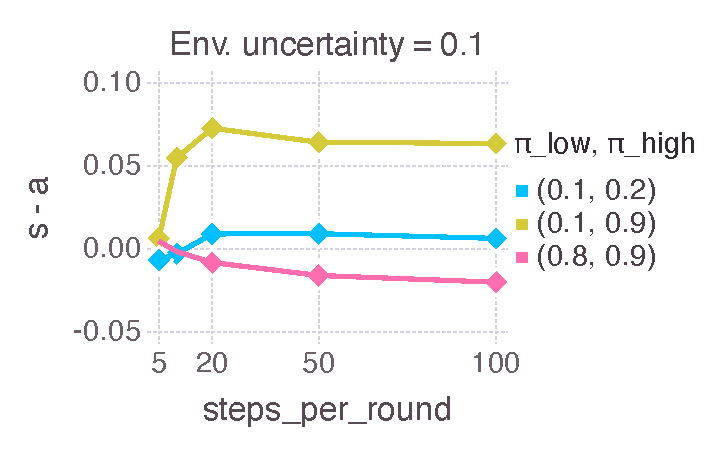
\includegraphics[width=\textwidth]{Figures/steps_per_round0p1.pdf}
  \caption{Low environmental uncertainty}
  \label{fig:steps_per_round0p1}
  \end{subfigure}
  \begin{subfigure}[b]{0.4\textwidth}
    \centering
  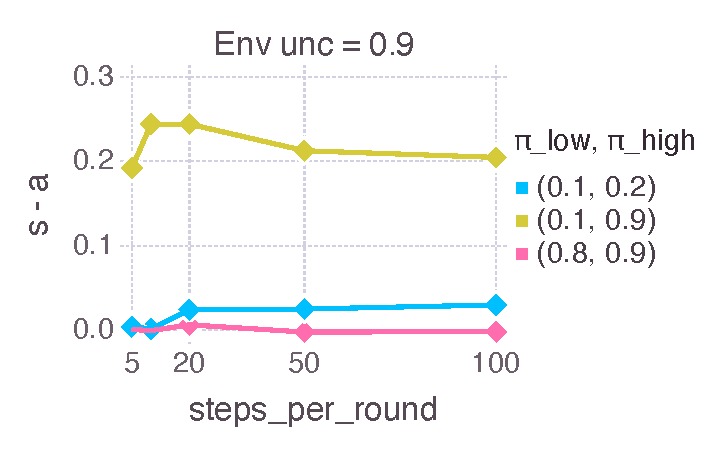
\includegraphics[width=\textwidth]{Figures/steps_per_round0p9.pdf}
  \caption{High environmental uncertainty}
  \label{fig:steps_per_round0p9}
  \end{subfigure}
  
\end{figure}





\bibliographystyle{apacite}

% \setlength{\bibleftmargin}{.125in}
% \setlength{\bibindent}{-\bibleftmargin}

\bibliography{/Users/mt/workspace/Writing/library.bib}

\end{document}
